\documentclass[a4paper,14pt]{extreport} %размер бумаги устанавливаем А4, шрифт 12пунктов
\usepackage[T2A]{fontenc}
\usepackage[utf8]{inputenc}%включаем свою кодировку: koi8-r или utf8 в UNIX, cp1251 в Windows
\usepackage[english,russian]{babel}%используем русский и английский языки с переносами
\usepackage{amssymb,amsfonts,amsmath,cite,enumerate,float} %подключаем нужные пакеты расширений
\usepackage[dvips]{graphicx} %хотим вставлять в диплом рисунки
\graphicspath{{images/}}%путь к рисункам
\usepackage{indentfirst}%отступ первого абзаца после названия главы

\makeatletter
\renewcommand{\@biblabel}[1]{#1.} % Заменяем библиографию с квадратных скобок на точку:
\makeatother

%для таблиц длиннее, чем на страницу
\usepackage{longtable}

%Добавляем "точки" после названий разделов
\usepackage{misccorr}

\usepackage{geometry} % Меняем поля страницы
\geometry{left=3cm}% левое поле
\geometry{right=1cm}% правое поле
\geometry{top=1.5cm}% верхнее поле
\geometry{bottom=2cm}% нижнее поле

%перечисления
%\renewcommand{\theenumi}{\arabic{enumi}}% Меняем везде перечисления на цифра.цифра
%\renewcommand{\labelenumi}{\arabic{enumi}}% Меняем везде перечисления на цифра.цифра
%\renewcommand{\theenumii}{.\arabic{enumii}}% Меняем везде перечисления на цифра.цифра
%\renewcommand{\labelenumii}{\arabic{enumi}.\arabic{enumii}.}% Меняем везде перечисления на цифра.цифра
%\renewcommand{\theenumiii}{.\arabic{enumiii}}% Меняем везде перечисления на цифра.цифра
%\renewcommand{\labelenumiii}{\arabic{enumi}.\arabic{enumii}.\arabic{enumiii}}% Меняем везде перечисления на цифра.цифра

\setcounter{secnumdepth}{3}% уровень вложенности счётчиков

%полуторный интервал между строками
%\renewcommand{\baselinestretch}{1.5}% вроде как плохой метод, т.к. растягивает заголовки и сноски, чего лучше не делать
\usepackage{setspace}
\onehalfspacing

%нумерация справа вверху
\usepackage{fancyhdr} 
\pagestyle{fancy} 
\lhead{} \chead{} \rhead{\normalsize\thepage}
\lfoot{} \cfoot{} \rfoot{}
\renewcommand{\headrulewidth}{0pt}
\renewcommand{\footrulewidth}{0pt}
\fancypagestyle{plain}{%
\fancyhf{} % clear all header and footer fields
\fancyhead[RE,RO]{\normalsize \thepage} % Even page, Odd page; Right, Left, Center
\renewcommand{\headrulewidth}{0pt}
\renewcommand{\footrulewidth}{0pt}
}

%попытка запилить Times New Roman
%\usepackage{pscyr}
%\renewcommand{\rmdefault}{ftm}
%\usepackage{mathptmx}
%\usepackage{cyrtimes}

\begin{document}
\begin{titlepage}
\newpage
\begin{center}
ФЕДЕРАЛЬНОЕ АГЕНТСТВО ПО ОБРАЗОВАНИЮ РФ \\
\vspace{1cm}
Московский авиационный институт \\*
(НАУЧНО-ИССЛЕДОВАТЕЛЬСКИЙ УНИВЕРСИТЕТ) \\*
\hrulefill
\end{center}
 
\flushright{КАФЕДРА \No 804}

\vspace{6em}

\begin{center}
\Large Пояснительная записка \\ к дипломному проекту на тему:
\end{center}

\vspace{2.5em}
 
\begin{center}
\textsc{\textbf{Моделирование времени ответа студента \linebreak в системах дистанционного обучения}}
\end{center}

\vspace{5em}
 
\begin{flushleft}
Студент \hrulefill Джумурат А. \\
\vspace{1.5em}
Научный руководитель \\
аспирант каф. 804 \hrulefill Иноземцев А.\\
\vspace{1.5em}
Рецензент \\
д.ф.-м.н., \hrulefill Наумов С.В.\\
\vspace{1.5em}
Зав. кафедрой \No 804 \\
д.ф-м.н, профессор \hrulefill Кибзун А.И.
\end{flushleft}
 
\vspace{\fill}

\begin{center}
Москва 2013
\end{center}

\end{titlepage} 
% это титульный лист
%Содержание
\renewcommand{\contentsname}{Содержание} 
%нумерация начинается со второй страницы
\setcounter{page}{2}
\tableofcontents % это оглавление, генерируется автоматически
{
\centering
\chapter{ОСНОВНАЯ ЧАСТЬ}
}
\setcounter{page}{4}
\newpage

\section{Введение в основную часть}
\label{intr}
\subsection{Актуальность дипломной работы}

В настоящее время одним из наиболее перспективных направлений раз\-вития в области образования является создание систем и методов дистанци\-онного обучения. Системы дистанционного обучения (СДО) позволяют ре\-шить проблему доступного образования: дистанционная модель (без присут\-ствия в образовательном учреждении) обеспечивает доступ к знаниям неза\-висимо места жительства и физических возможностей обучающегося. Сер\-висы дистанционного образования предоставляют как традиционные инсти\-туты (в России МГУ\cite{24.}, МИЛ\cite{25.}, МЭСИ\cite{26.}, за рубежом - MIT, Harvard, Stanford\cite{28.}), так и полностью виртуальные площадки в сети Интернет (Coursera\cite{27.}, Universarium\cite{29.} и т.д.).

В связи с развитием сервисов дистанционного обучения возникает необ\-ходимость в разработке математического и программного обеспечения для этих сервисов. Задачи, которые в возникают в данной области, а так же методы и пути их решения, получили название <<адаптивное компьютерное тестирование>> (Computer Adaptive Testing, CAT). Основной вопрос, на ко\-торый отвечают алгоритмы адаптивного компьютерного тестирования - как из пула задач подобрать задачу (или набор задач), которая максимально будет подходить для конкретного студента, т.е. СДО должна учитывать ин\-дивидуальные способности каждого обучающегося\cite{9.}. Такой подход к форми\-рованию индивидуального задания позволяет улучшить восприятие мате\-риала и способствует построению более эффективного процесса обучения.

Задача анализа времени ответа студента при ответе на задачи теста явля\-ется одним из приоритетных направлений области дистанционного обу\-чения и адаптивных систем тестирования. 

Время, которое студент затрачивает для ответа на задачу, является ос\-новным источником информации при ответе на следующие вопросы:
\begin{itemize}
\item не обладает ли студент ответами на некоторые (или все) задачи дистан\-ционного теста
\item достаточно ли отпущено времени для прохождения теста
\item удачно ли сформулированы задачи теста (или понимание условия за\-дачи вызывает затруднения)
\end{itemize}

На эти и некоторые другие вопросы помогает ответить стохастическая модель времени ответа в системах дистанционного обучения. Описанию такой модели и прикладных задач, которые решаются с её применением, посвящена данная дипломная работа.

{\itshape Объектом исследования} дипломной работы является поведение обуча\-ющихся при ответах на задания в системах дистанционного обучения. 

{\itshape Предметом исследования} дипломной работы является время, в течение которого студент отвечает на задачи, предлагаемые системой дистанционного обучения. 

\subsection{Цели и задачи}

Целью дипломной работы является адаптация системы дистанционного обучения на осно\-вании информации о времени, которое обучающийся затра\-чивает для ответа на задания теста

Основные задачи, которые необходимо решить для для достижения пос\-тавленной цели:
\begin{itemize}
\item ознакомление с теоретическим аспектом объекта исследования: поиск и чтение специализированной литературы
\item построение математической модели, описывающей предмет исследова\-ния
\item выбор методов оценки параметров построенных моделей
\item получение экспериментальных  данных
\item обработка данных моделирования эксперимента для оценки параметров математической модели
\item разработка алгоритма поиска отклонений в  новых данных, поступа\-ющих в систему дистанционного обучения, с помощью построенной мате\-матической модели для
\item описание и формализация задачи конструирования ограниченных по времени тестов заданной сложности.
\end{itemize}

Сформулированные задачи отражают процесс достижения поставленной цели дипломной работы.
%\subsubsection*{Элементы научной новизны в работе}

\subsection{Практическая значимость}

Дипломная работа имеет важное практическое приложение в качестве математического обеспечения для СДО МАИ CLASS.NET. Разработанные в работе методы и алгоритмы будут применяться для обеспечения учебного процесса пользователей данной системы.

В настоящее время созданию и развитию математического аппарата для СДО CLASS.NET посвящены работы \cite{14.,15.,16.}. Дипломная работа развивает идеи, предложенные в этих статьях, а так же предлагаются пути решения и формулировки для новых прикладных задач. 




\section{Аналитический обзор}
\label{mainpart} 
\subsection{Обзор объекта исследования}

Теоретические исследования в области построения математических моде\-лей процесса выполнения заданий играют огромную роль в современных системах компьютерного обучения. Одним из вопросов, которые исследуются в данной области, является взаимосвязь между временем ответа студента и корректностью ответа.

Наиболее ранние работы в данной области принадлежат Вудбори (Woodbury, 1951\cite{30.}, 1963\cite{31.}), который использовал стохастические модели для коли\-чества правильных ответов, предоставленных студентом в течение теста. Поз\-днее эти идеи были развиты в работах  Лорда и Новика (Lord, Novick, 1968\cite{32.}).

В этот период так же возникла идея о том, что оценка студента не должна складываться только из количества правильных ответов, предоставленных в течение теста - необходимо учитывать и время, которое студент затрачивает на решение задачи. Эти вопросы поднял в своих работах Галексен (Gulliksen, 1950\cite{33.}). Он предложил использовать два вида тестов - тесты на скорость (speed tests) и тесты на сложность задач (power tests). При прохождении теста на скорость студенту предлагалось за ограни\-ченное время решить макси\-мально возможное количество задач самого низ\-кого уровня сложности - таким образом Галексен пытался оценить скорость, с которой студенты принимают решения (при таком подходе на скорость ответов не должна влиять сложность задачи). Тесты второго вида состояли из задач разного уровня сложности, время на решение которых было неограничено - по результатам этого теста можно было оценить, задачи какого уровня сложности может решить студент, т.е. оценить именно уровень знаний, без привязки к скорости, с которой обучающийся решает задачи.

 Подход Галексена обладает двумя основными недостатками: во-первых, даже в тестах на скорость может случиться так, что на какую-то из задач студент даст неверный ответ (это маловероятно для студентов с высоким уровнем знаний, но вполне может произойти с менее способными студентами). Как в данном случае оценить скорость студента с помощью времени ответа, как учесть время, за которое студент дал неверный ответ и нужно его учиты\-вать вообще? Во-вторых, здравый смысл подсказывает, что время нужно учитывать так же и в тестах на сложность задач - ведь если два студента решают все предложенные задачи, но один из них при этом затрачивает меньшее количество времени - очевидно, что <<быстрый>> студент заслуживает более высокую оценку.

 Одним из первых исследователей, который пытался решить даные за\-дачи, был Терстоун (Thurstone, 1937\cite{34.}). Он обратил своё внимание на воп\-рос взаимосвязи между скоростью, с которой студент решает задачи теста, и уровнем знаний студента. Терстоун представил графическую модель такой взаимосвязи, которую назвал <<кривой ответа>> (response surface). Для каждого конкретного студента и одной задачи теста кривая ответа представляет собой график зависимости вероятности правиль\-ного ответа от сложности задачи и времени, которое было затрачено на ответ. 

\newpage
 Пример кривой ответа показан на рисунке \ref{respcurve}:

\begin{figure}[ht!] 
\centering \includegraphics[bb=0 0 450 228]{6.jpg} 
\caption{Кривая ответа}
\label{respcurve}
\end{figure}

График отражает зависимость между вероятностью правильного ответа и затраченным временем только для одного студента, т.е. не отражает распре\-деление вероятности для группы студентов. Основной принцип, который Тер\-стоун использовал при построении этой диаграммы: вероятность того, что студент даст правильный ответ на задачу растёт с увеличением времени, которое затрачено на решение задачи. При этом вероятность правиль\-ного ответа уменьшается с увеличением сложности задачи. Терстоун ввёл понятия ско\-рости студента и способностей студента. Скорость студентов Терстоун опре\-делил как число задач, которые студент решает в единицу времени; способ\-ностью студента исследо\-ватель назвал сложность задач, на которые студент отвечает с вероятностью $P=0.5$ при условии, что время ответа студента не ограничи\-вается.

Несмотря на достоинства, в модели Терстоуна есть так же и некоторые неочевидные недостатки. Во-первых, для ответов студента используется сто\-хастическая модель, а время ответа считается детерминирован\-ным. Очевидно, что и ответы студента, и время, которое студент затрачивает на ответ, являют\-ся следствиями одних и тех же когнитивных процессов - поэтому логично исполь\-зовать вероятностную модель так же и для времени ответа студента. Таким образом, кривая ответа должна преставлять собой закон совместного распределения времени ответа и корректности ответов сту\-дента. Во-вторых, модель Терстоуна принимает в качестве параметров веро\-ятностной модели ответа парамет\-ры задачи (сложность) и параметры сту\-дента (способность), при этом игнорируется время, в течение которого студент отвечал на задание. В-третьих, кривая ответа предполагает зависимость вероятности правильно\-го ответа от времени ответа, в то время как логично предположить, что между этими величинами существует условная незави\-симость, т.е. ответ на задачу и время ответа на любую задачу теста не должны зависеть от ответов на другие задачи для каждого студента.

Неторые эвристические модели для учёта времени ответа обучающихся во время тестирования были описаны в статье Вайса и Ма (Steven L. Wise and Lingling Ma, 2012\cite{18.}). Стохастические модели, которые включают время ответа студента, получили развитие в работах Гавирии (Gaviria, 2005\cite{17.}), который разработал логнормальную модель времени ответа. Большое коли\-чество работ посвящено поведению студентов во время теста и исследованию стратегий, которые обу\-чающиеся используют при ответе на задачи теста - например, работы Вайса и Конга (Wise and Kong, 2005\cite{19.}). Американские исследователи Ванг и Хансон (Wang and Hanson, 2001\cite{20.}) рассмотрели мо\-дель, включающую время ответа в качестве параметра, и разработали алго\-ритм, позволяющий в режиме реального времени конструировать вариант из пула задач с учётом индиви\-дуальных особенностей студента.

Таким образом, при изучении вопросов обучения студентов исторически возникли следующие задачи:
\begin{itemize}
\item оценить способность каждого студента
\item оценить скорость, с который конкретный студент может решить пред\-ложенную задачу теста
\item оценить время, которое может потребоваться студенту для полного про\-хождения теста
\item сформировать список задач, который будет оптимальным для конкрет\-ного студента, исходя из его способностей
\end{itemize}
и другие.

Дипломная работа посвящена построению математической модели вре\-мени ответа студента и двум практическим применениям этой модели: задаче выяв\-лении отклонений в поведении студента на основании поступающей в систему дистан\-ционного обучения информации о времени ответа студента на задачи теста для определения задач, к которым у студента заранее были ответы и задачи формирования индивидуального задания заданной слож\-ности для ограниченных по времени тестов. 

\subsection{Предмет дипломной работы}

Предметом дипломной работы является время, которое студент затрачи\-вает при ответе на вопросы теста. Очевидно, что время ответа играет важную роль при оценке уровня способностей студента и формирования индивидуаль\-ных заданий в системе дистанционного обучения: например, два студента с одина\-ковым уровнем подготовки  могут отвечать на вопросы теста с разной скоростью - это значит, что при одинаковых ограничениях на общее время на теста более <<медленный>> студент не успеет ответить на все задачи.

В связи с этим возникает необходимость в моделировании времени отве\-та студента. Информация о времени, которое ожидается при ответе обучающего\-ся на данную задачу, может использоваться системой дистанционного обуче\-ния для различных целей: например, для адап\-тации индивидуального зада\-ния согласно возможностям конкретного студента. Математическая модель вре\-мени ответа студента на задачи позволяет ответить на следующие вопросы:
\begin{itemize}
\item уложится студент во время, отведённое на тест для конкретного набора задач
\item не пытается ли студент во время теста угадать ответ вместо того, чтобы решать задачу
\item не пользуется ли студент готовыми решениями, полученными ранее
\item понять стратегию, которую студент использует  во время ответов на задачи
\item как сконструировать индивидуальное задание для онлайн форм кон\-троля, при выполнении которого студент уложится в заранее заданный временной интервал
\end{itemize}

Для решения этих задач существует множество теоретических моделей, которые рассматриваются далее, в разделе \ref{ch22}.

\chapter{Обоснование выбранного направления}
\label{ch22}
\section{Математические модели времени ответа}

Практика построения математических моделей, включающих время ответа, состоит из двух основных подходов. Первый поход - когда время ответа и распределение вероятности правильного ответа студента используются в одной и той же модели. Второй подход - когда используются разные модели. Приведём примеры для каждого подхода.

Во всех моделях, описанных далее, используются следующие обозначения:
$$
\begin{array}{lll}
j &-& \mbox{номер студента из группы}\\
i &-& \mbox{номер задачи из группы задач}\\
t_{ij} &-& \mbox{время ответа студента } i \mbox{ на задачу } j\\
\theta_j &-& \mbox{способность студента, уровень знаний}\\
b_i &-& \mbox{сложность задачи } i\\
u_{ij} &-& \mbox{случайная величина такая, что } u_{ij} = 1, \\  
& &\mbox{ если студент  j  ответил на задачу i верно} \\
c_i \in [0;1] &-& \mbox{вероятность угадать ответ на задачу } i
\end{array}
$$

\subsection{Модель корректности ответа, включающая время ответа}

Над моделью ответа, которая включает в себя время ответа, работал Роскам (Roskam) (1987). Эта модель является однопараметрической логистической моделью (1PL, one-para\-meter logistic):
\begin{equation}
p_i(\theta_j) = \{1+exp(-(\theta_j + \ln t_{ij} - b_j))\}^{-1}
\end{equation}

В этой модели $p_i(\theta_j)$ - вероятность правильного ответа. Модель отвечает идеям Терсто\-уна: для того, чтобы убедиться в этом, рассмотрим разность $\ln t_{ij} - b_j$. Увеличение сложнос\-ти задачи всегда может быть компенсировано более длительным временем, затра\-ченным на задачу.

\subsection{Модель времени ответа, включающая корректность ответа}

Модель такого типа разрабатывал, например, Гавирия (Gaviria) (2005):
\begin{equation}
\ln \left( \frac{t_{ij} - T_0}{A}\right) = -a_i(\theta_j - b_j) + \varepsilon_{ij},\; \varepsilon_{ij} \sim LN(0,\sigma_{i}^{2}),
\end{equation}
где
$$
\begin{array}{lll}
A &-& \mbox{параметр масштаба времени ответа}\\
T_0 &-& \mbox{параметр сдвига времени ответа}\\
\varepsilon_{ij} &-& \mbox{случайная ошибка, имеет логнормальное распределние}
\end{array}
$$

Таким образом, в модели Гавирии время ответа студента имеет логнор\-мальное распределение со средним $-a_i(\theta_j - b_j)$ и дисперсией $\sigma_{i}^{2}$, которая определяется параметрами задачи.

\subsection{Отдельные модели времени ответа и корректности ответа}

К таким моделям относится одна из самых ранних моделей в данной области - модель процесса чтения. Эту модель разработал Раш (Rasch) (1960). Модель включает в себя две модели более низкого уровня - модель ошибок в чтении и модель скорости чтения.
Модель ошибок описывается следующим образом: число ошибок чтения $a$ в тексте длиной $N$ слов имеет пуассоновское распределение, функция вероятности имеет вид
\begin{equation}
P(a | N) = e^{-\lambda}\frac{\lambda^a}{a!},
\end{equation}
где $\lambda = N\theta$ - среднее число ошибок. Раш рассматривал коэффициент $\theta$ как отношение
\begin{equation}
\theta = \frac{\delta_i}{\xi_j},
\end{equation}
где $\delta_i$ - сложность текста и $1/\xi_j$ - способность студента j.

Время, за которое текст будет прочитан студентом при этом имеет гамма-распределение с функцией плотности вероятности
\begin{equation}
\rho (t | N) = \lambda e^{-\lambda t}\frac{(\lambda t)^{N-1}}{(N-1)!},
\end{equation}
где $\lambda$ - параметр интенсивности потока, который соответствует скорости чтения студента.

Таким образом, обе модели представляют собой пуассоновские потоки разной природы - один поток для ошибок при чтении и второй поток для скорости чтения.

В дипломной работе приводятся принципы построения более сложной модели - \\двухуровневой модели Ван дер Линдена (van der Linden).

\section{Двухуровневая модель van der Linden'a}

При разработке двухуровневой модели оценки работы студента в системе \\дистанционного обучения использованы следующие предположения

\subsection{Базовые предположения}

\subsubsection{Случайное время ответа}

Исследования в области психологии доказывают, что время, в течении которого объект исследования реагирует на внешние раздражители, может быть случайным. Логично предположить , что время ответа студента в сис\-темах дистанционного обучения так же являтся случайной величиной. Ос\-новное предположение Теории ответов (ТО, Item Response Theory, IRT) со\-стоит в том, что корректность ответа студента является случайной величиной

{\itshape Предположение 1:} время ответа студента $t_{ij}$ является реализацией слу\-чайной величины $T_{ij}$

\subsubsection{Корректность ответов пользователя}

Для описания процесса обучения необходимо ввести ещё одну слу\-чайную величину - корректность ответа пользователя
$$
U_{ij} = 
\left\{
\begin{array}{ccl}
1 &,& \mbox{студент j ответил на задачу i корректно}\\
0 &,& \mbox{студент j ответил на задачу i некорректно}
\end{array}
\right.
$$

{\itshape Предположение 2:} корректность ответа студента $u_{ij}$ является реализацией случайной величины $U_{ij}$

\subsubsection{Скорость и время ответа}

Время, которое студент затрачивает при ответе на задачи теста и  скорость, с которой студент выполняет задание - неэквивалентные понятия. Одно из основных предположений в  Теории ответов - время ответа студента на задачу может меняться в зависимости от параметров задачи, в то время как скорость студента остаётся неизменной. Исходя из этого предположения, можно за\-писать {\itshape основное уравнение Теории ответов:}
\begin{equation}
\tau_{j}^{*} = \frac{\beta^{*}_{i}}{t_{ij}},
\end{equation}
где $\beta^{*}_{i}$ - трудозатраты, которые требуются от студента для решения задачи $i$ и $\tau_{j}^{*}$ - скорость студента.

Для того, чтобы распределение времени ответа имело более симметричный вид, к этому варажению обычно применяется лога\-рифмическое преобразо\-вание, тогда выражение при\-нимает вид
\begin{equation}
\ln {t_{ij}} = \beta_{i} - \tau_{j},
\end{equation}
где $\beta_{i} = \ln \beta^{*}_{i}$ и $\tau_{j} = \ln \tau^{*}_{j}$ - параметры в логарифмическом масштабе.

{\itshape Предположение 3:} время ответа на задания и скорость ответа студента на задание являются величинами разной природы, однако их связывает основное уравнение Теории ответов.

\newpage
\subsection{Описание модели}

\label{detmodel} 

На основании сделанных выше предположений, van der Linden предложил использовать для моделирования процесса обучения студента двухуровневую иерархическую модель. Модель имеет вид, представленный на диаграмме:

\begin{figure}[ht!] 
\centering \includegraphics[bb=0 0 450 351]{1.jpg} 
\caption{Двухуровневая иерархическая модель} 
\end{figure}

Как видно, модель имеет два уровня. На первом уровне вероятностные модели для корректности ответа студента и времени ответа студента. На втором уровне вероятностная модель распределения параметров студентов для всех групп обучающихся и вероятностная модель распределения слож\-ностных параметров задачи по всему пулу задач. Рассмотрим эти модели более подробно.

\subsubsection{Двухуровневая иерархическая модель}

\paragraph {Модель распределения параметров для множества студентов (верхний уровень)}

Параметры для группы студентов распределены по нормальному закону
\begin{equation}
(\theta,\tau) \sim N(\mu,\sigma),
\end{equation}
где $\mu = (\mu_\theta, \mu_\tau)^T$ и $\sigma=(\sigma_\theta,\sigma_\tau)$

\paragraph {Модель распределения параметров для множества задач (верхний уровень)}

Введём случайный вектор $\xi$ такой, что $\xi = (a_i,b_i,c_i,\alpha_i, \beta_i)$ - параметры задачи. Тогда
\begin{equation}
\xi \sim N(\mu,\Sigma),
\end{equation}
где $\mu$ - вектор мат. ожиданий и $\Sigma$ - ковариационная матрица для вектора  $\xi$

\paragraph {Модель корректности ответа (нижний уровень)}

Для модели кор\-ректности ответа используется трёхпараметрическая логистическая модель
\begin{equation}
p_i(\theta_j) = c_i - (1-c_i)\psi[a_i(\theta_j - b_i)]б
\end{equation}
где $\psi( * )$ - логистическая функция.

\paragraph {Модель времени ответа (нижний уровень)}
\label{mvonu}

Время ответа студента имеет \\логнормальное распределение:
\begin{equation}
\label{mainmodel}
\ln T_{ij} = \mu + \beta_i + \tau_j + \varepsilon_{ij},\quad \varepsilon_{ij} \sim N(0,\sigma^2).
\end{equation}
Соответственно, плотность распределения имеет следующий вид:
\begin{equation}
f(t_{ij};\tau_j,\alpha_i,\beta_i) = \frac{\alpha_i}{t_{ij}\sqrt{2\pi}}exp\left\{ -\frac{1}{2}[\alpha_i(\ln t_{ij} - \{\beta_i + \tau_j\})]^2 \right\},
\end{equation}
где $\alpha_i = \sigma^{-1}$

В модели используются следующие обозначения:
$$
\begin{array}{lll}
\beta_i &-& \mbox{временной параметр, индивидуальный для задачи i}\\
\tau_j &-& \mbox{параметр времени, в течении которого студент реагирует }  \\
& &\mbox{ на задачи теста }\\
\varepsilon_{ij} &-& \mbox{случайное отклонение}\\
\mu &-& \mbox{параметр времени, общий для всего пула задач и всех обучающихся}
\end{array}
$$

адаптация системы дистанционного обучения с использованием времени \\ответа обучающегося проходит с использованием модели (\ref{mainmodel})

\subsubsection{Оценка параметров модели}
\label{opm}

Пусть в сиcтеме дистанцинного обучения выбирает для формирования вариантов теста используется пул из $N$ задач. При этом в тестировании принимают участие $M$ студентов. Для каждого студента $j$ из общего числа студенов система дистанционного обучения формирует вариант из $n$ задач. Обозначим $t_{ij}$ этом время ответа студента $j$ на задачу $i$. Тогда для случайных параметров модели (\ref{mainmodel}) можно получить оценки методом макси\-мального правдоподобия:
\begin{equation}
\hat{\mu} = \frac{\sum\limits_{j=1}^{M}\sum\limits_{i=1}^{n}\ln t_{ij}}{n \cdot M},
\end{equation}
\begin{equation}
\hat{\beta}_i = \frac{\sum\limits_{j=1}^{M}\ln t_{ij}}{M} - \hat{\mu},
\end{equation}
\begin{equation}
\hat{\tau}_j = \frac{\sum\limits_{i=1}^{n}\ln t_{ij}}{n} - \hat{\mu},
\end{equation}
Оценка $\hat{\tau}_j$ имеет математическое ожидание
\begin{equation}
\label{exp}
E[\hat{\tau}_j] = \tau_j
\end{equation}
и дисперсию
\begin{equation}
\label{var}
Var(\hat{\tau}_j) = \frac{\sigma^2}{n}
\end{equation}
и, наконец, оценка для дисперсии случайного отклонения $\varepsilon_{ij}$ имеет вид
\begin{equation}
\hat{\sigma}^2 = \frac{\sum\limits_{j=1}^{M}\sum\limits_{i=1}^{n}\ln t_{ij} - \hat{\tau}_j - \hat{\beta}_i}{n \cdot M},
\end{equation}

\subsection{Прогнозирование времени ответа пользователя}

Для прогнозирования времени ответа в модели используется подход, опи\-санный ниже.

Обозначим прогнозное время ответа как $\tilde{T}_{ij}$. Тогда с учётом формул \\(\ref{exp}),(\ref{var}) получаем
\begin{equation}
\hat{\tau}_j \sim N\left(\tau_j, \frac{\sigma^2}{n-1}\right)
\end{equation}
т.к.
\begin{equation}
cov(\hat{\tau}_j,\varepsilon_{ij}) = 0,
\end{equation}
то получаем прогнозное время ответа студента на задачу
\begin{equation}
\label{predictedtime}
\ln \tilde{T}_{ij} \sim N\left(\mu + \beta_i + \tau_j,\frac{n\sigma^2}{n-1}\right)
\end{equation}

Таким образом, прогнозное время ответа студента на задачу имеет гаус\-совское распределение.
 \chapter{Методика исследования}

 \section{Использование информации о фактическом времени ответа}

Выражение для прогнозного времени ответа можно использовать для вы\-явления абер\-раций (отклонений) в поведении пользователя. Для этого введём понятие отклонения прогноза.

Отклонением прогноза будем разность между прогнозным временем ответа и фактичес\-ким временем ответа студента. В логарифмической шкале разность будет иметь вид отноше\-ния
\begin{equation}
E_{ij} = \ln \tilde{T}_{ij} - \ln t_{ij} =  \ln \frac{\tilde{T}_{ij}}{t_{ij}}
\end{equation}

Из этого отношения можно сделать вывод, что ошибка прогноза - случайная величина, которая имеет нормальное распределение c параметрами
\begin{equation}
E_{ij} \sim N\left(\mu + \beta_i + \tau_j - \ln t_{ij},\frac{n\sigma^2}{n-1}\right).
\end{equation}

Таким образом, выявление отклонений в поведении студента сводится к задаче проверки статистической гипотезы о том, что реализации $e_{ij}$ случайной величины $E_{ij}$ имеют нормаль\-ное распределение против альтернативы, что ошибка прогноза имеет какое-либо другое распреде\-ление
$$
\begin{array}{lll}
H_0 &:& e_{ij} \sim N\left(\mu + \beta_i + \tau_j - \ln t_{ij},\frac{n\sigma^2}{n-1}\right)\\
H_1 &:& \mbox{ошибка прогноза имеет другое распределение}
\end{array}
$$

\section{Обработка экспериментальных данных}

\subsection{Источник экспериментальных данных}

Для применения на практике теоретических положений и математических моделей, описанных в Главе \ref{ch22} использовались реальные данные пользователей системы дистанцион\-ного обучения МАИ. На момент написания диплома в системе не фиксировалось время, которое студент тратит на решение конт\-рольных и тестовых задач. В связи с этим в исходный код системы дистан\-ционного обучения и структуру базы данных, которая исполь\-зуется системой дистанционного обучения, были внесены доработки, позволяющие фикси\-ровать время ответа для всех существующих курсов (<<Математический ана\-лиз>>, <<Линейная алгебра и аналитическая геометрия>>, <<Теория вероятностей и математическая статистика>>).

После внесённых изменений система фиксирует следующие данные: сколь\-ко раз была отображена каждая задача, сколько попыток произвел каждый студент для её решения, какое количество времени было затрачено для каждой из попыток и насколько удачной была попытка (верно или неверно решена задача)

\subsection{Обработка полученных данных}

Для получения оценок параметров модели, описанных в разделе \ref{opm}, обработаем полученную статистику. Порядок обработки статистики покажем на примере задачи № 8.2.3 из курса <<Математический анализ>>

Вначале построим гистограмму для времени, которое студенты затра\-чивали для ответа на задачу
\begin{figure}[ht!]
\centering \includegraphics[scale=0.6]{test.eps}
\caption{Гистограмма времени ответа}
\end{figure}

Согласно модели, построенной в разделе \ref{mvonu}, применим логарифми\-ческое преобразование к времени ответа и построим гистограмму полученных значений:
\begin{figure}[ht!]
\centering \includegraphics[scale=0.6]{test1.eps}
\caption{Гистограмма времени ответа (логарифмический масштаб)}
\end{figure}

Как видно из данного примера, прменение логарифмического преобра\-зования к выборке по времени ответа обучающихся на конкретную задачу в системе дистанционного обучения позволяет получить симметричный вид распределения, который походит на гауссовское распределение. Проверка на гауссовость приводится в следующем пункте.

\subsection{Проверка предположения о гауссовости}

Проверим гипотезу о гауссовом распределении времени ответа студента. Для этого сформулируем основную и альтернативную гипотезы следующего вида:
$$
\begin{array}{lll}
H_0 &:& t_{ij} \sim N\left(\mu,\sigma^2\right)\\
H_1 &:& t_{ij} \mbox{ имеет другое распределение}
\end{array}
$$

\subsection{Оценка параметров модели по выборке}
\label{opmpv}

Проведём оценку параметров модели согласно пункту \ref{opm}.

\subsection{Применение модели к реальным данным}

Использя данные оценки, полученные в пункте \ref{opmpv}, продемонстрируем работу модели для выявления отклонений в поведении студентов.
\section{Содержание выполненной работы}

Выполненная дипломная работа состоит из двух основных разделов: тео\-ретической части работы и практической части работы.

В рамках теоретической части работы были проанализированы различные подходы, к исследованию времени, которое обучающийся тратит на ответ в системах компьютерного тестирования. Ряд подходов к данной проблеме  представлен в разделе \ref{ch22}. 

По результатам проведённого анализа в теоретической части работы для решения задачи, сформулированной в Введении, была выбрана одна из сос\-тавляющих двухуровневой иерархической модели ван дер Линдена - логнор\-мальная модель времени ответа.

Практическая часть выполненной работы состояла из двух основных час\-тей - это доработка существующей системы дистанционного обучения для решения задачи, постав\-ленной в дипломной работе, и получения эксперимен\-тальных данных для дальнейшей статистической обработки с целью оценки параметров модели. С использованием полученной модели был описан алго\-ритм выявления скомпроментированных задач.

Практическая часть работы включала в себя доработку системы дистан\-ционного обучения и обработку экспериментальных данных. В процессе ра\-боты над поставленной задачей возникла необходимость доработки сис\-темы дистанционного обучения. На момент написания дип\-ломной работы система дистан\-ционного обучения не производила учет вре\-мени, которое студент за\-трачивает при ответе на задачи в процессе работы с сис\-темой. Однако эта информация была нужна для проверки теоретических положений на практике. Для решения данной задачи были предприняты следующие шаги:

\begin{itemize}
\item построена диаграмма классов модуля системы дистанционного обучения
\item проанализаированы связи на диаграмме
\item спроектированы изменения, которые нужно внести в системы дистан\-ционного обуче\-ния для решения задачи
\item внесены изменения в программный код системы дистанционного обу\-чения
\end{itemize}

В результате произведённых действий в системе дистанционного обучения появилась возможность фиксировать время, которое студент затрачивает для ответа на задачи. Реализация указанных изменений была произведена с ис\-пользованиея языка веб-программирования PHP (который является основным языком разработки СДО МАИ CLASS.NET) и модификации базы данных MySQL, которую использует система.

При обработке экспериментальных данных были решены следующие за\-дачи:

\begin{itemize}
\item разработан алгоритм обращений к базе данных на языке запросов SQL
\item проведена первичная обработка экспериментальных данных
\item была проверена гипотеза о логнормальном распределении времени от\-вета
\item согласно разработанным алгоритмам была проведена оценка парамет\-ров модели
\end{itemize}

Для визуального анализа полученных статистических данных были пос\-троены гисто\-граммы. При статистической обработке данных использовался язык программирования Python и библиотека статистических методов stats.py.

\section{Задача конструирования ограниченных по времени тестов}

В качестве одного из приложений построенной модели можно привести задачу формирования индивидуальных заданий для ограниченных по вре\-мени тестов. Для корректной оценки знаний учащихся необходимо проведение ру\-бежного контроля, который включает в себя задачи разных типов. Обычно время проведения рубежного контроля ограничено - поэтому важно подобрать задачи таким образом, чтобы студенту хватило времени для его прохожения. Вероятностная модель времени ответа позволяет конструировать задания, которые учитывают индивидуальные особенности студентов.

Описаннная проблема сводится к следующей задаче линейного програм\-мирования с вероятностным ограничением (задача решается для конкретного студента, т.е. примем $t_{ij} \sim t_i$ для кратковсти):

$$
\left \{
\begin{array}{ll}
c-\sum\limits_{i=1}^{n}w_ix_i \rightarrow min & \\
\sum\limits_{i=1}^{n} x_i = k & \mbox{// количество задач в индивидуальном задании}\\
c - \sum\limits_{i=1}^{n} x_i \ge - \varepsilon & \mbox{// допустимая погрешность}\\
c - \sum\limits_{i=1}^{n} x_i \le \varepsilon & \mbox{// допустимая погрешность}\\
P\left( \sum\limits_{i=1}^{n} x_i t_{i} \le T \right) \ge \alpha & \mbox{// вероятностное ограничение на время теста}
\end{array}
\right.
$$

где

$$
\begin{array}{lcl}
c & - & \mbox{ требуемая сложность задания}\\
k & - & \mbox{ число задач в задании}\\
n & - & \mbox{ общее количество задач в пуле}\\
w_i & - & \mbox{ сложность задания i }\\
x_i & - & \mbox{ принадлежность задачи i тесту}\\
i & - & \mbox{ номер задания }, i=1,\ldots,K\\
j & - & \mbox{ номер студента, для которого генерируется задание}, j=1,\ldots,M\\
K & - & \mbox{ количество задач в пуле}\\
M & - & \mbox{ количество пользователей}
\end{array}
$$

Переменная $x_i$ является бинарным признаком принадлежности задачи тесту в следующем смысле:
$$
x_i = 
\left\{
\begin{array}{ll}
1, \mbox{ задача i попала в индивидуальное задание}\\
0, \mbox{ задача i не попала в индивидуальное задание}
\end{array}
\right.
$$

Так как случайные величины $t_{i}$, которые входят в вероятностное ограни\-чение,  распределены нормально и закон их распределения известен, то для данной задачи в стохастической по\-становке можно выписать детерминиро\-ванный эквивалент\cite{38.}:

$$
\left \{
\begin{array}{l}
c-\sum\limits_{i=1}^{n}w_ix_i \rightarrow min \\
\sum\limits_{i=1}^{n} x_i = k \\
c - \sum\limits_{i=1}^{n} x_i \ge - \varepsilon \\
c - \sum\limits_{i=1}^{n} x_i \le \varepsilon \\
\sum\limits_{i=1}^{n} x_{i}m_{i}  + \Phi^{-1}(1-\alpha)\sqrt{\sum\limits_{i=1}^{n} x_{i}^{2}\sigma^{2}_{i}} \le T 
\end{array}
\right.
$$
где $\Phi(x)$ - функция Лапласа. Т.к. время ответа имеет логнормальное распре\-деление, то и линейная комбинация (которая входит в вероятностное ограниче\-ние) так же распре\-делена нормально.
 \section{Результаты}
 \label{ch5}

В дипломной работе приведены предпосылки к необходимости модели\-рования времени, которое студент затрачивает при ответе на задачи в системе дистанционного обучения. Формулируется математическая вероятностная мо\-дель времени ответа, для которой приводятся аналитические оценки пара\-метров.

Корректность модели и степень её применимости проверяется на реальных данных СДО МАИ CLASS.NET. Для этого в программный код системы вносятся изменения для получения необходимой статистической информации о пользователях. Внесённые доработки позволя\-ют фиксировать время ответа студента и сохранять его для дальнейшей обработки. Добавлением новых таблиц изменена структура базы данных, а так же модифицирован алго\-ритм внесения информации о работе пользователя в БД. Разработана программная библиотека на языке программирования Python для доступа к базе данных и работы со статистической информацией. По результатам обработки экспе\-риментальных данных был сделан вывод о соот\-ветствии математической мо\-дели и реальных данных СДО МАИ CLASS.NET.

Согласно сформулированной математической модели была произведена оценка параметров по реальным данным с использованием разработанного программного модуля. Была разработана процедура прогнозирования вре\-мени ответа пользователя.

По результатам сравнивания прогнозных значений с фак\-тическими про\-изводится вывод о том, не обладал ли студент ответами к решаемой задаче. Описан алгоритм принятия решения, использующий понятие доверительного интервала.

На основании решения о компроментации задачи можно принимать раз\-личные административные решения: назначить пользователю решение до\-полнительных задач, убрать скомпроментированные задачи из пула для дан\-ной группы студентов и т.д.

В качестве одного из приложений описанной математической модели при\-ведена задача конструирования ограниченных по времени тестов с учётом индивидуальных способностей студента.
\chapter{Заключение} 

Задачи, сформулированные в разделе <<Введение>> выполнены: построена математическая модель времени ответа студента, на основании модели была решена задача прогнозирования времени ответа студента. По результатам прогноза описан алгоритм выявления откло\-нений при ответе на задачи с целью определить случаи, когда  студент имеет готовые ответы на одну или несколько задач теста.

Математическая модель получила программную реализацию и была при\-менена данным, полученным в системе дистанционного обучения МАИ.

Прогнозирование времени ответа студента является важной частью адап\-тивного компьютерного тестирования. Полученные результаты (математиче\-ская модель и программная реализация) могут быть применены не только к выявлению случаев мошенничества при прохождении тестирования, но и в ряде других задач: прогнозирование времени, которое понадобится студенту для прохождения теста; оценка вероятности выполнения теста в срок; про\-верка того, как формулировка задания влияет на скорость выполнения и выбор оптимальной формулировки.
 \chapter{ЭКОНОМИЧЕСКИЙ РАЗДЕЛ}
 \setcounter{page}{32}
\newpage

 \section{Введение в экономический раздел}

Целью дипломной работы является доработка системы дистанционного обучения МАИ с целью адаптации системы на основе поступающей инфор\-мации о времени, которое студент затрачивает для ответов на задачи в про\-цессе тестирования. На основании анализа времени ответа делается вывод о том, не было ли у студента заранее приготовленных ответов не задачи теста.

В основной части диплома описывается математическое обеспечение сис\-темы и программная реализация, которые в совокупности представляют со\-бой завершенный программный продукт, готовый для продажи на рынке программного обеспечения.

В экономической части диплома производится расчёт затрат, которые несёт заказчик программного обеспечения системы дистанционного обучения МАИ. Исходя из затрат формируется стоимость проекта. По результатам оценки стоимости проекта производится расчёт экономической эффективно\-сти. Так же на основании сетевого графика производится расчёт временных па\-раметров проекта и вероятность его успешного выполнения в установлен\-ный срок.

\section{Сетевой график}

Сетевой график представляет собой графическое отображение этапов ра\-бот, которые необходимо провести для завершения дипломного проекта. С помощью сетевого графика можно спрогнозировать общее время, которое потребуется для выполнения проекта, а так же вычислить вероятность вы\-полнения проекта в срок.

\subsection{Таблица этапов работ}
По каждому этапу дипломной работы указано минимальное время выпол\-нения этапа и максимальное время выпол\-нения этапа. Исходя из этих зна\-чений рассчитывается ожидаемое время, которое потребуется затратить на данный этап:
$$
t_{exp} = \frac{2t_{min}+3t_{max}}{5}
$$

Дисперсия времени работы вычисляется по формуле
$$
t_{exp} = \left( \frac{t_{max} - t_{min}}{5} \right)^2
$$

По результатам расчётов построим таблицу
%\begin{myTable}
\begin{center}
Таблица 2.2: Таблица этапов работ
\end{center}
{
\scriptsize
\begin{longtable}[H]{|p{0.9cm}|p{3.4cm}|p{1.4cm}|p{3.9cm}|p{0.6cm}|p{0.7cm}|p{0.6cm}|p{0.7cm}|}
%\caption{\normalsize Таблица этапов работ}}\\
\hline
Этап & Событие             & Шифр & Работа                                        & $t_{min}$ & $t_{max}$ & $t_{exp}$ & $\sigma$\\
\hline
1    & Изучение литературы & 1-4  & Изучение литературы по основной части диплома & 2         & 5         &  3,8      &  0,36    \\
\cline{3-8}
& &1-12&Изучение литературы по экономической части&3&6&4,8&0,36\\
\cline{3-8}&&1-10&Изучение литературы по охране труда и окружающей среды&1&4&2,8&0,36\\
\hline
2&Окончание доработки СДО&2-7&Анализ структуры и программного кода СДО&6&9&7,8&0,36\\
\hline
3&Получен список необходимых доработок&3-2&Доработка СДО для получения экспериментальных данных и оценки параметров модели&4&8&6,4&0,64\\
\hline
4&Необходимость построения математической модели&4-5&Изучение математических методов моделирования времени ответа в СДО&2&5&3,8&0,36\\
\hline
5&Завершение математической модели&5-6&Применение математической модели для анализа времени ответа&7&11&9,4&0,64\\
\cline{3-8}
&&5-2&Описание математической модели&6&9&7,8&0,36\\
\hline
7&Оценка параметров модели&7-8&Оценка по экспериментальным данным параметров модели &7&10&8,8&0,36\\
\cline{3-8}
&&7-9&Применение модели к реальным входным данным&2&5&3,8&0,36\\
\hline
8&Прогнозирование ответа на основании модели&8-9&Получение результатов обработки реальных данных&3&6&4,8&0,36\\
\hline
9&Построение таблиц, диаграмм, анализ полученных данных&9-14&Оформление результатов практической части&4&7&5,8&0,36\\
\hline
10&Раздел <<Охрана труда и окружающей среды>>&10-11&Написание теоретического материала раздела <<Охрана труда и окружающей среды>>&3&5&4,2&0,16\\
\hline
11&Расчет кондиционирования&11-14&Проведение расчётов&6&8&7,2&0,16\\
\hline
12&Раздел <<Экономическая эффективность>>&12-13&Написание теоретического материала раздела <<Экономическая эффективность>>&2&5&3,8&0,36\\
\hline
13&Построение сетевого графика&13-14&Проведение расчётов&6&9&7,8&0,36\\
\hline
14&Оформление готового диплома&-&Оформление полученных результатов&&&&\\
\hline
\end{longtable}
}
%\end{myTable}

\newpage

\subsection{Построение сетевой модели}

Построим на основании таблицы из п. (1.2.1) «Таблица этапов работ» сетевой график. Круги обозначают события, стрелками обозначены работы. Подписи над стрелками указывают ожидаемое время выполнения работы.
\\
\begin{figure}[ht!]
\label{setgr}
\centering 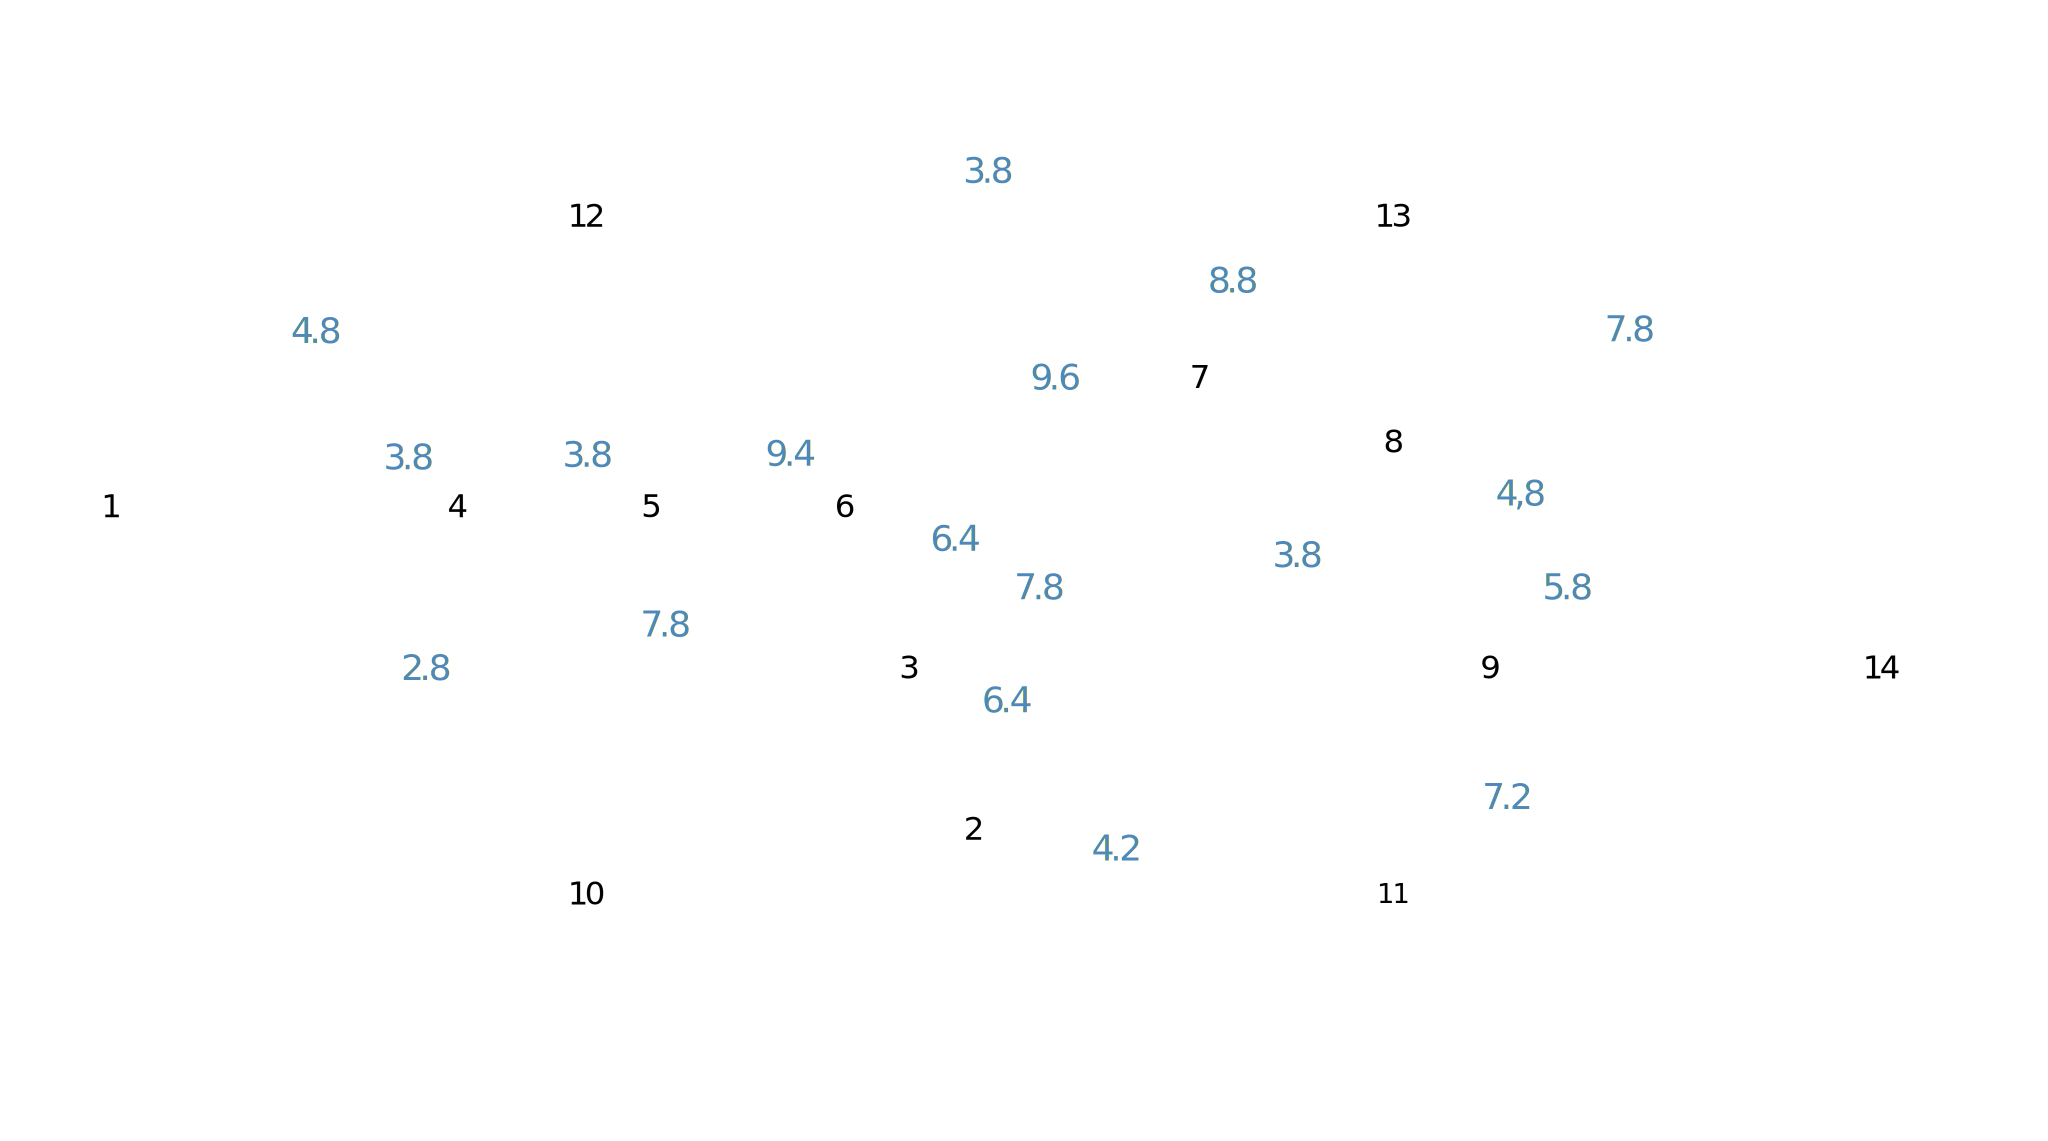
\includegraphics[bb=0 0 437 243]{Setevoy_Grafik.jpg}
\caption{Сетевой график}
\end{figure}
\\
\subsection{Анализ сетевой модели.}

{\itshape Путём} в сетевой модели называется последовательность работ, соединя\-ющая две любые работы на графике (если такая последовательность сущест\-вует).
Введём обозначения: $L_{1(i)}$ - путь, предшествующий событию $i$, $L_{2(i)}$ - путь, следующий за событием $i$.

Критический путь на сетевой модели (последовательность событий от начала проекта к концу проекта, имеющая максимальную длину):
$$
L = 1-4-5-6-3-2-7-8-9-14
$$

Длина пути $T(L) = \sum\limits_{i-j}t_{i-j}$ (где $t_{i-j}$ - длительность работы с меткой $i-j$) - сумма длительностей работ, которые выполняются при следовании по пути. Длина критического пути:
$$
T_{\mbox{кр}}(L) = 3.8+3.8+9.4+6.4+6.4+7.8+8.8+4.8+5.8 = 57 \mbox{ дней}
$$
Ранний срок наступления события: $t_{\mbox{р}(i)} = max(T(L_{1(i)}))$\\
Ранний срок начала работы: $t_{\mbox{рн}(i-j)} = max(T(L_{1(i)}))$\\
Ранний срок окончания работы: $t_{\mbox{ро}(i-j)}= t_{\mbox{р}(i)} - t_{(i-j)} = max(T(L_{1(i)})) + t_{(i-j)} $\\
Поздний срок наступления события: $t_{\mbox{п}(i)}= T_{\mbox{кр}}(L) -  max(T(L_{2(i)}))$\\
Поздний срок начала работы: $t_{\mbox{пн}(i-j)}= t_{\mbox{по}(i)} - t_{(i-j)}$\\
Поздний срок окончания работы: $t_{\mbox{по}(i-j)} = t_{\mbox{п}(j)}= T_{\mbox{кр}}(L) -  max(T(L_{2(i)}))$\\
Общий резерв времени работы: $R_{(i-j)} = t_{\mbox{по}(i-j)} - t_{\mbox{ро}(i-j)} =  t_{\mbox{п}(j)} -  t_{\mbox{р}(j)} -  t_{(i-j)}$\\
Свободный резерв времени работы: $r_{(i-j)} = t_{\mbox{р}(i-j)} - t_{\mbox{ро}(i-j)} =  t_{\mbox{р}(j)} -  t_{\mbox{р}(i)} -  t_{(i-j)}$\\
Резерв времени события: : $r_{(i)} = t_{\mbox{п}(i)} - t_{\mbox{р}(i)} $

Результат расчёта параметров для сетевой модели работы над дипломным проектом представлен в таблице:

\begin{center}
Таблица 2.3: Параметры сетевой модели
\end{center}
{
\footnotesize
\begin{longtable}[H]{|p{1.1cm}|p{0.5cm}|p{0.5cm}|p{1.1cm}|p{1.1cm}|p{1.1cm}|p{1.1cm}|p{0.9cm}|p{0.9cm}|p{0.9cm}|}
%\caption{Параметры сетевой модели \label{psm}}\\
%\caption{\label{psm}}\\
\hline
Шифр & $t_{exp}$ & $\sigma$ &  $t_{\mbox{рн}(i-j)}$ $t_{\mbox{р}(i)}$ & $t_{\mbox{ро}(i-j)}$ & $t_{\mbox{пн}(i-j)}$ & $t_{\mbox{по}(i-j)}$ $t_{\mbox{п}(j)}$ & $R_{(i-j)}$ & $r_{(i-j)}$ & $r_{(i)}$\\
\hline
1-4&3,8&0,36&0&3,8&8,8&12,6&8,8&0&8,81\\
\hline
1-12&4,8&0,36&0&4,8&49,4&54,2&49,4&0&49,4\\
\hline
1-10&2,8&0,36&0&2,8&51,6&54,4&51,6&1,4&51,6\\
\hline
2-7&7,8&0,36&29,8&37,6&38,6&46,4&8,8&0&8,8\\
\hline
3-2&6,4&0,64&23,4&23,4&32,2&38,6&15,2&6,4&15,2\\
\hline
4-5&3,8&0,36&3,8&7,6&12,6&16,4&8,8&2,7&8,8\\
\hline
5-6&9,4&0,64&7,6&17&16,4&25,8&8,8&9,6&8,8\\
\hline
5-2&7,8&0,36&15,4&15,4&30,8&38,6&23,2&14,4&23,2\\
\hline
6-3&6,4&0,64&17&23,4&25,8&32,2&8,8&0&8,8\\
\hline
6-7&9,6&0,04&26,6&26,6&36,8&46,4&19,8&11&19,8\\
\hline
7-8&8,8&0,36&37,6&46,4&46,4&55,2&8,8&0&8,8\\
\hline
7-9&3,8&0,36&37,6&51,2&56,2&60&8,8&0&8,8\\
\hline
8-9&4,8&0,36&46,4&51,2&55,2&60&8,8&0&8,8\\
\hline
9-14&5,8&0,36&51,2&57&60&65,8&8,8&0&8,8\\
\hline
10-11&4,2&0,16&2,8&7&54,4&58,6&51,6&0,2&51,6\\
\hline
11-14&7,2&0,16&7&14,2&58,6&65,8&51,6&0&51,6\\
\hline
12-13&3,8&0,36&4,8&8,6&54,2&58&49,4&0&49,4\\
\hline
13-14&7,8&0,36&8,6&16,4&58&65,8&49,4&0&49,4\\
\hline
\end{longtable}
%\end{myTableSecond}
}

Директивный срок выполнения проекта составляет 122 дня, при этом длина критического пути 57 дней – таким образом, проект будет завершён в срок и нет необходимости перестраивать сетевой график проекта. Сумма дисперсий работ, лежащих на критическом пути, составляет 4.08. Среднеквад\-ратическое отклонение для критического пути составляет $\sqrt{4.08} = 2.02$ . Доверительный интервал для срока выполнения всех работ имеет вид $[50.6-2.02,50.6+2.02 ] \sim [30.58, 52.62]$. Вероятность выполнения работы в срок составляет $P=\Phi((122-50.6)/2.02)=\Phi(35.3)\sim 1$, где $\Phi(x)$ – функция Лапласа.

\section{Расчет затрат}
\label{rz}

В разделе описаны основные затраты разработчика, влияющие на це\-ну конечного продукта: расходные материалы, аренда помещений, зара\-ботная плата и т.д.

\subsection{Материальные}

Для выполнения дипломного проекта требуется приобрести следующие материальные активы: шариковые ручки, бумагу формата А4, картридж для принтера, скрепки для степлера. Количество материалов, а так же их стоимость приведены в таблице \ref{materials}:

\begin{table}[H]
\caption{Материалы \label{materials}}
\begin{center}
\begin{tabular}{|p{3.5cm}|p{3.6cm}|p{3.6cm}|p{3.4cm}|p{3.4cm}|}
\hline
Товар & Цена (руб.) & Количество (шт.) & Сумма (руб.)\\
\hline
Ручка &40 &5 &200\\
\hline
Скрепки &2 &20 &40 \\
\hline
Файл для бумаг &3 &10 &30\\
\hline
Пачка бумаги А4(200шт) &150 &1  &150\\
\hline
Картридж &400 &4 &1600\\
\hline
\multicolumn{3}{|c|}{Итого}& 2020 \\
\hline
\end{tabular}
\end{center}
\end{table}

Таким образом, материальные затраты на написание диплома составляют $M=2020$ руб.

\subsection{Заработная плата}
\label{zp}

При работе над экономической частью дипломного проекта необходимо рассчитать заработную плату сотрудникам, задействованным в работе над дипломом.

В работе над дипломным проектом принимают участие научный руково\-дитель, студент, консультанты. Для каждого специалиста вычисляется объём заработной платы, исходя из почасовой ставки и  времени, в течение которого специалист участвует в проекте.

Расчёты приведены в таблице \ref{zp2013}, данные по заработной плате научных ру\-ководителей и консультантов соответствуют зарплатам в Московском авиа\-ционном институте за 2013 г. Оплата для студента, выполняющего дипломную работу, соответствует размеру стипендии.
\begin{table}[H]
\caption{Заработная плата \label{zp2013}}
\begin{center}
\begin{tabular}{|p{3.5cm}|p{1.8cm}|p{1.6cm}|p{2.8cm}|p{2.1cm}|p{1.8cm}|}
\hline
Специалист&Заработ\-ная плата&Коли\-чество часов &Количество часов на одного дипломника&Почасовая оплата&Заработ\-ная плата\\
\hline
Научный руководитель&40000&90&24&444&10666\\
\hline
Консультант по экономической части&40000&90&2&444&888\\
\hline
Консультант по охране труда и окружающей среды&40000&48&2&833&1666\\
\hline
Студент&3000&-&-&-&12000\\
\hline
\multicolumn{5}{|c|}{Итого}&25220\\
\hline
\end{tabular}
\end{center}
\end{table}

Итого затраты на заработную плату составят Z = 25220 руб.

\subsection{Расходы на амортизацию оборудования}

Оборудование, которое использовалось в ходе выполнения дипломной ра\-боты, подлежит амортизации. Амортизации подвергаются основные средства и нематериальные активы для переноса части их стоимости в цену произво\-димой продукции.

Основным оборудованием (средством производства) является ноутбук DE\-LL Vostro 1440 стоимостью N = 21459 руб. Расчет амортизации произведём линейным способом:
$$
A = \frac{S\cdot n \cdot t}{ 100 \cdot T}
$$

В таблице \ref{ammort} приведены расшифровка и значения переменных формулы:
\begin{table}[H]
\caption{Амортизация оборудования \label{ammort}}
\begin{center}
\begin{tabular}{|p{3.0cm}|p{3.8cm}|p{2.6cm}|}
\hline
Переменная&Описание&Значение\\
\hline
S&Стоимость оборудования&21459 руб.\\
\hline
n&Годовая норма амортизации&20 \%\\
\hline
t&Время работы оборудования&252 часа\\
\hline
T&Эффективный срок работы оборудования&1800 часов\\
\hline
\end{tabular}
\end{center}
\end{table}

Произведём расчёт согласно данным таблицы:
$$
A = \frac{21459\cdot 20 \cdot 252}{ 100 \cdot 1800} = 601 \mbox{ (руб.)}
$$

Таким образом, амортизация ноутбука за период написания диплома со\-ставит 601 руб.

\section{Социальные отчисления}

Работодателю необходимо произвести социальные отчисления с зарплаты работников в следующем размере:
\\
Взносы в ФФОМС: 5.1\%\\
Взносы в ФСС: 2.9\%\\
Взносы в Пенсионный фонд: 22\%

Таким образом, на затраты на социальные отчисления составят (с учётом фонда оплаты труда из пункта \ref{zp} «Заработная плата»)
$$
P = Z \cdot (5.1 + 2.9 + 22)\% = Z \cdot 30 = 25220 \cdot 30\% = 7566 \mbox{ (руб.)}
$$

Итого, размер социальных выплат составит $7566$ руб.

\section{Прочие расходы}

\subsection{Транспортные расходы}

Затраты на транспорт фигурируют в работе над дипломным проектом, т.к. встречи между участниками проекта происходят на территории МАИ и каждый из работников затрачивает денежные средства на то, чтобы добрать\-ся до института. Предполагается, что все участники добираются до на метро.

В таблице \ref{transport} для каждого участника учтено количество поездок (опреде\-ляется исходя из этапов работы над дипломом), а так же полные затраты на транспорт за период написания диплома:
\begin{table}[H]
\caption{Транспортные расходы \label{transport}}
\begin{center}
\begin{tabular}{|p{3.5cm}|p{2.8cm}|p{2.6cm}|p{2.8cm}|}
\hline
Специалист&Количество поездок&Стоимость 1-ой поездки&Итого\\
\hline
Научный руководитель&16&&448\\
\cline{1-2}\cline{4-4}Консультант по экономической части&2&&56\\
\cline{1-2}\cline{4-4}Консультант по охране труда и окружающей среды&2&28&56\\
\cline{1-2}\cline{4-4}Студент&20&&560\\
\hline
\multicolumn{3}{|c|}{Итого}&1120\\
\hline
\end{tabular}
\end{center}
\end{table}

Итого расходы на транспорт составляют M = 1120 руб.

\subsection{Связь}

К прочим расходам относятся так же расходы на мобильную связь. Исходя из того, что стоимость одного комплексного тарифного плана оператора со\-товой связи <<МТС>>, включающего 300 минут разговоров и неограниченное количество смс составляет 500 руб. для каждого участника разработки дип\-лома, то за 4 месяца для 4-х человек получаем
$$
B = 500 \cdot 4 \cdot 4 = 8000 \mbox{ (руб.)}
$$

Итого, расходы на связь составляют 8000 руб.

\subsection{Интернет}

Ежемесячная абонентская плата за Интернет составляет 200 руб, общая продолжительность дипломного проекта составляет 4 месяца. Таким образом, затраты на Интернет в течение периода составляет
$$
S = 200 \cdot 4 = 800
$$

Итого, расходы на Интернет составляют $S = 800$ руб.

\subsection{Электроэнергия}

Тарифы на электроэнергию в Москве составляют 4р/КВтч. Ежедневное энергопотребление работающего компьютера составляет 50 КВт за 4 часа работы. С учётом 7-ми дневной рабочей недели, получаем за 4 месяца. 
$$
E = 50 \cdot 7 \cdot 4 \cdot 4 = 11200
$$

Таким образом, окончательно получаем
$$
Y = 800 + 8000 +1120 + 11200= 21120
$$

Итого, прочие расходы составляют 21120 руб.


\section{Расчет экономической эффективности}

Для расчёта экономической эффективности нужно вычислить себесто\-имость продукта, его цену продажи, а так же экономический эффект, который ожидается от внедрения продукта

\subsection{Расчёт цены на продукт}

Чтобы рассчитать цену на продукт, необходимо вычислить его себесто\-имость. Себестоимость продукта с определяется как сумма всех затрат, вы\-численных в пункте \ref{rz} «Расчет затрат».\\
\begin{math}
SS = M + Z + A + P + Y = \\ 
= 2020 + 25220 + 601 + 7566 + 21120 = 56527 \mbox{ руб.}
\end{math}

Норма прибыли равна 5\%. НДС, который так же нужно учесть в цене, составляет 18\%. Тогда цена на продукт составит
$$
C = 56527 \cdot (100\% + 5\% + 18\%) = 63876 \mbox{ (руб.)}
$$

\section{Экономический эффект}

Экономический эффект, который принесёт внедрение доработок в систему дистанционного обучения, заключается в ликвидации недополученной при\-были за дополнительные занятия для студентов.

После внедрения системы появится возможность выделить среди группы студентов, проходящих курсы в системе дистанционного обучения, тех поль\-зователей, которые решают задачи теста с заранее имеющимися ответами.

Если студент использует  готовые ответы – он не до конца освоил нужный курс и нуждается в дополнительных занятиях. Оценим прибыль, которую институт может получить за один семестр по формуле:
$$
L = N \cdot i \cdot k \cdot V
$$

\newpage
В таблице \ref{profit} приведены расшифровка и значения переменных в формуле.
\begin{table}[H]
\caption{Экономический эффект\label{profit}}
\begin{center}
\begin{tabular}{|p{3.0cm}|p{4.1cm}|p{2.6cm}|}
\hline
Переменная&Описание&Значение\\
\hline
N&Количество студентов &430\\
\hline
i&Доля воспользовавшихся ответами&15 \%\\
\hline
k&Стоимость одного доп. занятия на курсах&540 руб.\\
\hline
V&Количество доп. занятий&4 шт\\
\hline
\end{tabular}
\end{center}
\end{table}

Таким образом, получаем:
$$
L = N \cdot i \cdot k \cdot V = 450 \cdot 15 \cdot 540 \cdot 4 =  139320 \mbox{ (руб.)}
$$

Итого, экономический эффект от модификации системы дистанционного обучения сос\-тавит 139320 руб в семестр.

\subsection{Экономическая эффективность}

Для расчёта экономической эффективности необходимо учесть расходы на внедрение системы и эксплуатацию сервиса.

Расходы на внедрение системы  вычисляются по формуле 
$$
C_{\mbox{вн}} = t_{\mbox{вн}}\cdot p,
$$
где $t_{\mbox{вн}} = 3$ часа - время, необходимое для установки системы на сервер и $p=630$ руб - почасовая ставка программиста, который занимается развёр\-тыванием системы
$$
C_{\mbox{вн}} = 3 \cdot 630 = 1890 \mbox{ (руб.)},
$$

Расходы на эксплуатацию сервиса складываются из затрат на оплату сервера, который использует система дистанционного обучения:
$$
C_{\mbox{эксп}} = t_{\mbox{эксп}}\cdot c,
$$

где $t_{\mbox{эксп}} = 6$ мес. (расчёты производим за семестр) и  $c = 1200$ руб. – помесячная оплата сервера. Тогда
$$
C_{\mbox{эксп}} = 6 \cdot 1200 = 7200 \mbox{ (руб.)}.
$$ 

Итого получаем срок окупаемости вложенных средств:
$$
T_{\mbox{ок}} = \frac{C_{\mbox{эксп}} + C_{\mbox{вн}} + C}{L} = \frac{7200+1890+63876}{139320} = 0.52 (\mbox{ семестра})
$$

Таким образом средства, вложенные в систему, будут возвращены в течение половины семестра.

\section{Вывод} 
В экономической части дипломной работы был произведён расчёт се\-бестоимости и цены продажи проекта.

Построен сетевой график выполнения дипломной работы. По графику найден критический путь и рассчитаны параметры сетевой модели для каж\-дого узла. По рассчитанным параметрам произведена оценка наиболее веро\-ятного срока выполнения проекта, а так же вычислена вероятность завер\-шения проекта в срок.

Была проведена оценка затрат на введение и эксплуатацию системы, а так же оценка прибыли, которую принесёт проект. На основании этих данных определена экономическая эффективность разработанной системы.

По результатам расчётов сделан вывод о том, что вложенные в систему средства будут возвращены инвестору в течении половины учебного семестра.
 \chapter{Охрана труда и окружающей среды}
\label{mainpart}  
\section{Введение}

\subsection{Необходимость защиты труда в объекте дипломной работы}

Дипломная работа посвящена анализу времени, которое затрачивает обу\-чающийся при ответе на задачи в системе дистанционного обучения. Одно из достоинств электронной версии методических и учебных материалов состоит в том, что студент может проходить обучение как в домашней обстановке, так и на территории института (в компьютерном классе). 

Как известно, на скорость студента при ответе влияет не только способ\-ность самого студента к обучению, но и факторы помещения, в котором проходит процесс обучения, - отсюда следует, что при проведении занятий на территории института необходимо  обеспечить в помещениях, где проходит работа с системой дистанционного обучения, условия для продуктивной ра\-боты. Необходимо учесть вредные факторы, которые могут возникнуть у студентов в процессе работы и устранить эти факторы, а так же причину их возникновения

\subsection{Характеристики рабочего помещения}
\label{hro}

Рабочее помещение, в котором проводятся занятия, имеет следующие ха\-рактеристики:

\begin{itemize}
\item {\itshape длина,} м : 10
\item {\itshape ширина,} м : 15
\item {\itshape площадь,} м$^2$ : 150
\item {\itshape высота,} м : 5
\item {\itshape рабочих мест,} шт. : 20
\item {\itshape площадь на одного студента,} м$^2$. : 7,5
\item {\itshape объём на одного студента,} м$^3$. : 37,5
\end{itemize}

\subsection{Характеристики оборудования}

Помещение, в котором проводятся занятия, оснащено персональными ком\-пьютерами в следующей комплектации:
\begin{itemize}
\item системный блок (основные комплектующие, производящие шумовое воз\-действие – вентилятор и жесткий диск)
\item клавиатура
\item мышь
\item соединительные провода
\item монитор
\end{itemize}

Каждое рабочее место оснащается одним персональным компьютером.

В таблице приведён уровень шума и мощность для каждого комплек\-тующего

\begin{table}[H]
\begin{center}
\begin{tabular}{|l|c|c|}
\hline
Комплектующее &Уровень шума(дБ) & Мощность оборудования(Вт)\\
\hline
Жесткий диск & 35 & 10\\
\hline
Вентилятор & 40 & 15\\
\hline
Клавиатура & 0 &  0.75\\
\hline
Мышь & 0 & 1 \\
\hline
Соединительные провода & 0 & 0.1 \\
\hline
Монитор & 15 & 25\\
\hline
\end{tabular}
\end{center}
\end{table}

\section{Анализ условий труда}

\subsection{Санитарно-гигиенические факторы}
\label{sangen}

\subsubsection{Микроклимат}

Микроклимат - искусственно создаваемые условия микросреды в зак\-рытых помещениях.
Микроклимат необходимо поддерживать, для создания комфорт\-ных условий работы - влажности, скорости движения воздуха, тем\-пературы, давления и т.д.

Для обеспечения нормального микроклимата применяются:

\begin{itemize}
\item кондиционирование
\item вентилирование
\item обогрев
\end{itemize}

Требования к микроклимату определяет ГОСТом 30494-96 «Здания жи\-лые и общест\-венные. Параметры микроклимата в помещениях»  и ГОСТом 12.01.005-88 «Общие санитарно-гигиенические требования к воздуху рабочей зоны». Учебные аудито\-рии согласно ГОСТу относятся к помещениям 2-ой категории/

Согласно классификации, приведённой в ГОСТ 12.01.005-88, работа с сис\-темой дистан\-ционного обучения, относится к категории работ 1а – это лёгкие работы, т.е. работы, производимые сидя и сопровождающиеся незначитель\-ным физическим напряжением.

В таблице приведены нормативные значения и фактические значения в помещении, где проходит работа с сис\-темой дистанционного обучения:

\begin{table}[H]
\begin{center}
\begin{tabular}{|l|p{1,3cm}|p{2.7cm}|p{3.2cm}|p{3cm}|}
\hline
Период года &  & Температура воздуха $^\circ$С & Относительная влажность, \% & Скорость движения воздуха, м/с(не более)\\
\hline
Холодный & ГОСТ & 22-24 & 40-60 & 0.1\\
%\cline{2-5}
 & Факт & 26 & 55 & 0.05\\
\hline
Тёплый & ГОСТ & 23-25 & 40-60 & 0.1\\
%\cline{2-5}
 & Факт & 27 & 60 & 0.08\\
\hline
\end{tabular}
\end{center}
\end{table}

Таким образом, фактические условия микроклимата в помещении, где используется система дистанционного обучения, не соответствуют требова\-ниям ГОСТ. 12.01.005-88, поэтому необходимо рассчитать параметры кондици\-онирования для устранения негативных факторов.

\subsubsection{Освещение}

Правильно спроектированное и рационально исполненное освещение помо\-гает создать комфортные психофизиологические условия для длительной работы - поэтому освещён\-ность является одним из важнейших факторов для комфортного протекания про\-цесса обучения. Для улучшения видимости объектов освещение должно быть рав\-номерным. Так же в поле зрения сту\-дента не должно быть резких переходов от света к тени. Большое количество глянце\-вых поверхностей по возможности нужно заменить матовыми, чтобы избежать блёсткости.

Нормы освещения в образовательных помещениях определяются СанПиН\\ 2.2.1/2.1.1.1278-03 «Гигиенические требования к естественному, искусствен\-ному и сов\-мещенному освещению жилых и общественных зданий». В по\-мещении используется совме\-щенный комбинированный тип освещения. Срав\-ним фактические показатели со стан\-дартом:

\begin{table}[H]
\begin{center}
\begin{tabular}{|p{3cm}|p{3cm}|p{3cm}|}
\hline
& \multicolumn{2}{|c|}{Освещённость (лк)}  \\
\cline{2-3}
& всего & в т.ч. от общего \\
\hline
СанПиН & 500 & 300\\
\hline
Факт & 510 & 305\\
\hline
\end{tabular}
\end{center}
\end{table}

Показатели помещения соответствуют значениям СаНПиН 2.2.1/2.1.1.1278-03 и в корректировке не нуждаются.

\subsubsection{Электроопасность}

Действие электрического тока на организм может быть разнообразным: ожоги, механи\-ческие повреждения кожи, изменение биологических процессов организма.

Электротравмы  подразделяются на общие и местные. Общая травма – это электри\-ческий удар. Приводит к судорогам, остановке дыхания, нарушению сердечной деятель\-ности. К местным травмам относят ожоги (термические повреждения), металлизацию кожного покрова, механические повреждения тканей (разрыв тканей в результате  электро\-динамического эффекта).

Для гигиенического нормирования электроопасности оборудования ис\-пользуется ГОСТ 12.1.038-82, «Электробезопасность. Предельно допустимые значе\-ния напряжений  прикос\-новения и токов», который устанавливает пре\-дельно допустимые токи, протекающие через тело человека во время при\-косновения к электроустановкам.
При работе с системой дистанционного обу\-чения в сис\-темных блоках протекает переменный ток частотой 50 Гц. Для такого уровня тока при действии в течении 0.6 сек. ГОСТ 12.1.038-82 опреде\-ляет предельно допустимый уровень напряжения в 125 В. При этом напря\-жение на корпусе системного блока составляет 100 В – таким образом, требо\-вания ГОСТ соблюдены.

\subsubsection{Шум}

Звук - это акустические колебания упругой среды. {\itshape Акустическими} на\-зывают колебания, которые может воспринять человек с нормальным слухом, т.е. колебания в диапазоне частот $16$ Гц - $209$ кГц. Звуковые колебания, распро\-страняющиеся в пространстве, предста\-вляют собой акустическое поле.

{\itshape Шумом} называют совокупность акустических звуков различной интен\-сивности и часто\-ты (см. \cite{10.}). Интенсивный шум на производстве является негативным фактором: шум способстует увеличению числа ошибок в процессе работы, так как приводит к снижению внимания. Так же шум негативно влияет на скорость принятия решений, затрудняет протекание аналитических процессов.

В биологическом отношении шум представляет собой стрессовый фактор, который может вызвать срыв припособительных способностей организма, т.н. акустический стресс. Акустический стресс может приводить к разнообразным расстройствам, от расстройств центральной нервной системы до морфоло\-гический деструктивных изменений в органах и тканях. Степень негативного влияния шума зависит от продолжительности воздействия, уровня интенсив\-ности шума, функционального состояния нервной системы человека и индиви\-дуальной чувствительности конкретного человека в данному виду раздражи\-теля (что очень важно - например, женский и детский оргаизм более чувстви\-тельны к шуму). Высокая индивидуальная чувствительность к шуму может становиться причиной развития неврозов, других расстройств нервной сис\-темы, а так же быстрой утомляемости.

Шум оказывает сильное влияние различные аспекты функционирования организма человека: угнетение ЦНС, нарушение дыхания, сбои пульса, может стать причиной нарушения обмена веществ, возникновению сердечно-сосу\-дистых заболеваний, развитию различных профессиональных болезней.

Уровень звукового давления принято измерять в децибелах (дБ). Децибелл - отно\-сительная единица измерения звукового давления. Измерение уровня звука проиcходит по отношению к опорному давлению $p_0=20$ мкПа, которое соответствует порогу слы\-шимости синусоидальной звуковой волны частотой $1$ кГц. Уровень звукового давления в децибеллах $N$ для давления $p$ вычисля\-ется по формуле
$$
N = 20 \log \frac{p}{p_0}
$$

Особо выделяют следующие уровни шума:
\begin{itemize}
\item {\itshape 30 \ldots 35} дБ : привычен для человека и не беспокоит его;
\item {\itshape 40 \ldots 70} дБ : возникает значительная нагрузка на нервную систему, ухудшение самочувствия;
\item {\itshape 70 \ldots 140} дБ : может привести к потере слуха;
\item {\itshape 140 \ldots 160} дБ : разрыв барабанных перепонок и контузия;
\item свыше {\itshape  160} дБ : смерть.
\end{itemize}

Норму параметров шума на рабочих местах определяет ГОСТ 12.1.003-831 «Шум. Общие требования безопасности» с дополнениями 1989 г. Документ классифицирует шумы по спектру (широкополосные и тональные) и по вре\-менным характеристикам (постоянные и непостоянные). Для нормирования постоянных шумов используются допустимые уровни звукового давления \\(УЗДН) в девяти активных полосах частот, разделённых по видам произ\-водственной деятельности. В свою очередь непостоянные шумы делятся на три груп\-пы:

\begin{itemize}
\item колеблющиеся
\item прерывистые
\item импульсные
\end{itemize}

Сравним фактические данные с нормами ГОСТ 12.1.003-83 на рабочих местах, связа\-нных с обучением. Для этого произведём расчёт фактического уровня шума согласно таблице пункта \ref{hro}

Произведём расчёт звукового давления оборудования по каждому источ\-нику:
$$
\mbox{Жесткий диск: } p_1= 10^{35/20}\cdot 2 \cdot 10^{-4} = 0.01
$$
$$
\mbox{Вентилятор: } p_2= 10^{40/20}\cdot 2 \cdot 10^{-4} = 0.02
$$
$$
\mbox{Монитор: } p_3= 10^{15/20}\cdot 2 \cdot 10^{-4} = 0.001
$$

С учётом проведённых расчётов, вычислим результирующий уровень шу\-ма:
$$
N = 20 \log \frac{\sum\limits_{n}^{i=1}p_i}{p_0} =  20 \log \left(\frac{0.01 + 0.02 + 0.001}{2 \cdot 10^{-4}}\right) = 
$$
$$
=  20 \log \frac{0.031}{2 \cdot 10^{-4}} = 44 \mbox{ дБ}
$$

Проверим полученный результат на соответствие ГОСТ

\begin{table}[H]
\begin{center}
\begin{tabular}{|p{4cm}|p{3cm}|}
\hline
Деятельность: обучение & Уровень шума (дБ)  \\
\hline
ГОСТ & 50  \\
\hline
Факт & 44  \\
\hline
\end{tabular}
\end{center}
\end{table}

Таким образом, фактический уровень шума соответствует нормативному.

\subsubsection{Вибрация}

Вибрации - это механические колебания, которые возникают и распро\-страняются в упругих средах. Воздействие вибрации на человека разделяют по способу передачи коле\-баний (общая и локальная), по направлению дей\-ствия (по оси $x$, по оси $y$, по оси $z$) и по временным характеристикам (по\-стоянная, непостоянная).

Между частотой воздействующей вибрации и реакциями организма нет линейной зави\-симости. Причина - в эффекте резонанса. Если внешняя частота вибраций совпадает с собственными вибрация тела, воздействие становится крайе негативным.

Особенно сильное воздействие вибрация оказывает на зрение. Расстрой\-ство зрительного восприятия происходит при частотном диапазоне от $60$ до $90$ Гц. Патологии, связанные с вибрацией по количеству связанных с ними профес\-сиональных заболеваний стоят на втором месте после пылевых патологий.

Так же при действии вибрации на организм страдает нервная система, вестибюлярный и тактильный анализаторы. У людей, длительное время под\-вергающихся вибрации, отме\-чают головокружения, снижение остроты зрения.

Гигиеническое нормирование вибрации производится на основании ГОСТ 12.1.012-90 <<Вибрационная безопасность. Общие требовани>> (воспользуемся эквивалентными скор\-ректированными значениями).

\begin{table}[H]
\begin{center}
\begin{tabular}{|p{4.1cm}|p{2cm}|p{1cm}|p{2cm}|p{1cm}|}
\hline
Среднегеометрические частоты полос, Гц & \multicolumn{4}{|c|}{Допустимые значения по осям $X_0, Y_0, Z_0$  } \\
\cline{2-5}
       & \multicolumn{2}{|l|}{виброускорения                   }&\multicolumn{2}{|l|}{ виброскорости                    } \\
\cline{2-5}
       & $10^{-3} \mbox{ м}^2 / \mbox{с}$  & дБ & $10^{-3} \mbox{ м}^2 / \mbox{с}$  & дБ   \\
\hline
СанПиН & 10                                & 80 & 0.28                              & 75   \\
\hline
Факт   & 9.8                               & 77 & 0.25                              & 70   \\
\hline
\end{tabular}
\end{center}
\end{table}

Таким образом, значения вибрации соответствуют нормам ГОСТ.

\subsubsection{Электромагнитные излучения}

В зависимости от энергии фотонов выделяют ионизирующие и неиони\-зирующие излу\-чения. Среди неионизирующих в свою очередь выделяют элек\-трические и магнитные поля.

Нормирование ЭМИ промышленной частоты производится путём уста\-новления допус\-тмых уровней напряжённости электрического поля $E$(кВ/м) и напряженности маг\-нитного поля $H$(А/м).

Пребывание в электрическом поле напряжённостью до $5$ кВ/м допускается в течении всего рабочего дня. Допустимое время (в часах) пребывания в ЭП напряжённостью $5 \ldots 10$ кВ/м вычисляется по формуле
$$
T = \frac{50}{E} - 2,
$$
где $E$ - напряжённость воздействующего поля в контролируемой зоне, кВ/м.

Нормирование значение напряженности определяется СанПиН 2.2.4.1191-03 <<Электро\-магнитные поля в производственных условиях>>. Т.к. металличес\-кий корпус системного блока экранирует магнитные поля и прошел соответ\-ствующую сертификацию на стороне производителя, то нормы СанПиН вы\-полняются.

\subsection{Эргономика рабочего места}

\label{erg}

Требования к эргономике рабочего места закреплены в санитарно-эпиде\-миологических нормах СанПиН 2.2.2/2.4.1340-03 <<НАЗВАНИЕ>>. Рабочее место студента должно отвечать требованиям, обеспечивающим достаточную степень эрго\-номичности. Для обеспечения этих требований должны выполняться опре\-делённые условия: 
\begin{itemize}
\item оптимальное раcположение оборудования;
\item достаточный объём рабочего пространства.
\end{itemize}

Рабочее место студента, оснащённое персональным компьютером, имеет следующие параметры эргономики: 
\begin{itemize}
\item высота рабочей поверхности должна регулироваться в пределах $680-850$ мм, при отсутствии регулировки — 725мм
\item размеры пространства для ног должны не должны вызывать диском\-форт
\item расположение документов на рабочем месте
\item Кресло должно быть подъемно-поворотным, регулируемым по высоте, углам наклона сиденья и спинки
\item поверхность рабочего стола
\item возможность регулировки элементов рабочего места
\end{itemize}

Удобная рабочая поза студента помогает избежать перенапряжения мышц и спо\-собствует улучшению кровотока и дыхания. При неудобной рабочей позе могут появиться боли в мышцах, суставах и сухожилиях. Так же среди программистов, проводящих большое количесто времени на неэргономичном рабочем месте, развивается туннельный синдром запястья.
Правильное по\-ложение в рабочем кресле включает в себя:
\begin{itemize}
\item прямую посадку
\item опора - только на спинку кресла
\item расслабленную позу без излишнего напряжения в поясничном отделе
\item голова  - немного наклонена (до 20 градусов)
\item руки расслаблены, локти держать под углом 90 градусов, кисти рук — на уровне локтей или немного ниже
\item колени должны быть на уровне бедер, стопы - на подставке
\end{itemize}

Соблюдение норм эргономики, описанных выше, позволит снизить вред\-ное воздействие ЭВМ на пользователя персонального компьютера, повысить вни\-мательность, снизить наг\-рузки на зрительные и слуховые рецепторы.

\subsection{Психофизиологические факторы}

К психофизиологическим факторам относятся перегрузки (физические и эмоциональ\-ные), перенапряжение связанное с интеллектуальной работой и монотонностью труда. Психофи\-зиологические факторы могут вызывать перенапряжение как в физическом, так и в интел\-лектуальном плане.

Оценка психофизиологических факторов проводится с помощью руковод\-ства P2.2.2006-05 <<Руководство по гигиенической оценке факторов рабочей среды и трудового процесса. Критерии и классификация условий труда>>

В руководстве P2.2.2006-05 под пунктом 5.10. <<Тяжесть и напряженность трудового процесса>> с помощью Таблицы 18 <<Классы условий труда по по\-казателям» напряженности трудового процесса» определим класс физичес\-кого труда>>.

Проведём анализ класса условий труда с использованием соответству\-ющих таблиц руководства P2.2.2006-05:

\begin{longtable}[H]{|p{5.5cm}|p{6cm}|p{3.0cm}|}
\hline
Показатель & Значение & Класс условий труда \\
\hline
\multicolumn{3}{|l|} {1.Интеллектуальные нагрузки:}\\
\hline
1.1. Содержание работы & Решение простых задач по инструкции & Допустимый \\
\hline
1.2.Распределение функций по степени сложности задания & Обработка, выполнение задания и его проверка & Допустимый\\
\hline
1.3.Характер выполняемой работы & Работа по установленному графику с возможной его коррекцией по ходу деятельности & Допустимый\\
\hline
\multicolumn{3}{|l|} {2.Сенсорные нагрузки}\\
\hline
 2.1.Длительность сосредоточенного наблюдения(\%времени)&26-50&Допустимый\\
\hline
2.2.Наблюдение за экранами видеотерминалов (часов)& до З &Допустимый\\
\hline
\multicolumn{3}{|l|} {3.Эмоциональные нагрузки}\\
\hline
З.1.Степень ответственности за результат собственной деятельности. Значимость ошибки& Несет ответственность за функциональное качество выполения заданий. Влечет за собой дополнительные усилия со стороны преподавателя&Допустимый\\
\hline
3.4.Количество конфликтных ситуаций (за занятие)&1-3&Допустимый\\
\hline
\multicolumn{3}{|l|} {4. Монотонность нагрузок}\\
\hline
4.1. Число элементов (приемов), необходимых для реализации простого задания или в многократно повторяющихся операциях&более 10&Оптимальный\\
\hline
4.2. Продолжительность (в сек) выполнения простых заданий или повторяющихся операций& более 100&Оптимальный\\
\hline
4.3. Время активных действий (в \% к продолжительности смены). В остальное время – наблюдение&19 - 10&Допустимый\\
\hline
Монотонность производственной обстановки (время пассивного наблюдения), \% &76–80&Допустимый\\
\hline
\end{longtable}

Согласно таблицам, класс труда определяем как «Допустимый». Этот уровень соответ\-ствует напряжённости труда средней степени.

\section{Расчёт}

Согласно СНиП 41-01-2003 «Отопление, вентиляция и кондиционирование воздуха», расход воздуха на одного человека в помещениях, находящихся в общественных зданиях без естественного проветривания составляет 60 м$^3$/ч. Исходя из этой нормы, рассчитаем величину кондиционирования по формуле (СНиП 41-01-2003? Приложение М, формула И.1), используя величину из\-бытков явной теплоты:
$$
L = L_{w,z} + \frac{3.6Q - cL_{w,z}(t_{w,z} - t_{in})}{c(t_{l}-t_{in})},
$$
где

$L_{w,z}$ - расход воздуха, удаляемого из обслуживаемой или рабочей зоны помещения системами местных отсосов, и на технологические нужды,  $\mbox{м}^3/\mbox{ч}$

$Q$ - избыточный явный тепловой поток в помещении, ассимилируемый воздухом центральных систем вентиляции и кондиционирования, Вт

$t_{w,z}$ - температура воздуха, удаляемого системами местных отсосов в об\-служиваемой или рабочей зоне помещения, и на технологические нужды, $^\circ$C

$t_{in}$ - температура воздуха, подаваемого в помещение $^\circ$C

$t_{l}$ - температура воздуха, удаляемого из помещения за пределами обслу\-живаемой или рабочей зоны, $^\circ$C

$c$ - теплоемкость воздуха, равная 1,006 $\mbox{кДж}/(\mbox{кгС})$

Произведём расчёт избыточного теплового потока Q. Избыточный тепло\-вой поток определяется по формуле
$$
Q = Q_{ob} + Q_{l} + Q_{os} + Q_{ok},
$$
где 

$Q_{ob}$ - теплота, выдёляемая оборудованием. В соответствии с характерис\-тиками обору\-дования из пункта 1.1.3 «Характеристики оборудования», по\-лучаем.
$$
Q_{ob} = P_{ob}\cdot f = (10+15+0.75+0.1+0.25)\cdot 0.25 = 13 \mbox{ Вт},
$$
где

$P_{ob}$ - номинальная мощность оборудования (Вт), $f=0.25$ - коэффициент передачи

 $Q_{l}$ -теплота, выделяемая людьми в помещении. При этом $Q_{l} = 50\cdot \frac{1000}{860} = 58 \mbox{Вт}$, т.к. один человек выделяет $50 \mbox{ ккал/час}$

$Q_{os}$ - теплота, выделяемая системой освещения
$$
Q_{os} = P_{os} \cdot a \cdot b \cdot \cos(f) = 20 \cdot 4 \cdot 0.46 \cdot 1 \cdot 0.3 = 11 \mbox{Вт},
$$
где

$a = 0.46$ - коэффициент перехода электрической энергии в световую

$b = 1$ -  коэффициент одновременной работы ламп

$\cos(f) = 0.3$ - коэффициент мощности

$P_{os} = 20 \mbox{ Вт}$ -  номинальная мощность освещения одной лампы освещения
(всего таких ламп 4 шт.)

$Q_{ok}$ - теплота, выделяемая ограждающими конструкциями
$$
Q_{ok} = F\cdot q_{ok} = 18 \cdot 11 \cdot \frac{1000}{860} = 230 \mbox{ Вт},
$$
где

$F = 18 \mbox{ м}^2$  - площадь ограждающей конструкции, излучающей тепло

$q_{ok} = 11 \mbox{ ккал/м}^2$ -  теплота, которую излучает 1 м$^2$ ограждающей кон\-струкции.

Таким образом, получаем избыточный тепловой поток
$$
Q = Q_{ob} + Q_{l} + Q_{os} + Q_{ok}= 13 + 58 + 11 + 230 = 312 \mbox{Вт}
$$

Рассчитаем требуемую величину кондиционирования:
{\small
$$
L = L_{w,z} + \frac{3.6Q - cL_{w,z}(t_{w,z} - t_{in})}{c(t_{l}-t_{in})} = 2 + \frac{3.6\cdot312\cdot3600 - 1006\cdot2\cdot(22-19)}{1006(24-19)} = 804
$$
}

Согласно произведённым расчётам и ГОСТ 26963—86 <<Кондиционеры бытовые авто\-номные. Общие технические условия>>, необходимо выбрать сле\-дующий кондиционер: тип КБ1 и климатическое исполнение У3, обозначение климатического исполнения по ГОСТ 15150-69 «Исполнение для различных климатических районов».

\section{Вывод}

Помещение, которое используется для обучения студентов с использо\-ванием системы СДО отвечает условиям безопасности труда - это подтвер\-ждается проведёнными расчётами. 

Согласно произведённым расчётам рекомендуется выбрать кондиционер КБ1 У3, тогда параметры микроклимата в помещении будут соответствовать принятым нормам.


 

\input{Outro}
%меняем "Литература" на корректное название
\renewcommand{\bibname}{Список использованных источников}
\addcontentsline{toc}{chapter}{Список использованных источников}

\begin{thebibliography}{2}
\bibitem{1.}{\itshape Wim J. van der Linden}  Some New Developments in Adaptive Testing Technology / Journal of Psychology 2008 Vol. 216(1), pp. 3–11
\bibitem{2.}{\itshape Rob R. Meijer, Leonardo S. Sotaridona}  Detection of Advance Item Knowledge Using Response Times in Computer Adaptive Testing/ Law School Admission Council Computerized Testing Report; 2006
\bibitem{3.}{\itshape Wim J. van der Linden}  A Lognormal Model for Response Times on Test Items / Journal of Educational and Behavioral Statistics; 2006, Vol. 31, No. 2, pp. 181–204
\bibitem{4.}{\itshape Wim J. van der Linden} Modeling response times with latent variables: Principles and applications/ Psychological Test and Assessment Modeling, Vol. 53, 2011 (3), pp. 334-358
\bibitem{5.}{\itshape Wim J. van der Linden, Edith M.L.A. Van Krimpen-Stoop} Using Response Times to Detect Aberrant Responses in Computerized Adaptive Testing / Psychometrika Vol. 68, No. 2, 251-265
\bibitem{6.}{\itshape Wim J. van der Linden, David J. Scrams, Deborah L. Schnipke} Using Response-Time Constraints to Control for Differential Speededness in Computerized Adaptive Testing / Applied Psychological Measurement, Vol. 23 No. 3, September 1999, 195–210
\bibitem{7.}{\itshape Wim J. van der Linden}  Predictive Control of Speededness in Adaptive Testing/ Law School Admission Council Computerized Testing Report; 2007
\bibitem{8.}{\itshape Wim J. van der Linden}  Conceptual Issues in Response-Time Modeling / 
\bibitem{9.}{\itshape Wim J. van der Linden}  Using Response Times for Item Selection in Adaptive Testing / Journal of Educational and Behavioral Statistics March 2008, Vol. 33. No. 7, pp. 5-20
\bibitem{10.}{\itshape С.В. Белов, В.А. Девисилов, А.В, Ильницкая и др.}  Безопасность жизнедеятельность / М.: Высш. шк., 2007
\end{thebibliography}
\end{document} 
